\section{Fourier}
\subsection{Harmonics}
\begin{itemize}
    \item $y=A_1\sinn{x}$ is the first/fundemental harmonic
    \item $y=A_n\sinn{nx}$is the $n^{\text{th}}$ harmonic
\end{itemize}
\subsection{Periodic Function}
A function is periodic if:
\begin{equation}
    \f{x+P}=\f{x},\quad\text{where }P=\text{period}
\end{equation}
\subsection{Fourier Series}
\subsubsection{Arbitrary Period, $2L$: $\bracket{-L\leq x\leq L}$}
Fourier series, $\f{x}$:
\begin{equation}
    f\bracket{x}=\frac{a_0}{2}+\sum_{n=1}^\infty\cbracket{a_n\cos\bracket{\frac{n\pi x}{L}}+b_n\sin\bracket{\frac{n\pi x}{L}}}
\end{equation}
Constant $a_0$:
\begin{equation}
    a_0=\frac{1}{L}\int_{-L}^Lf\bracket{x}dx
\end{equation}
Constant $a_n$:
\begin{equation}
    a_n=\frac{1}{L}\int_{-L}^Lf\bracket{x}\cos\bracket{\frac{n\pi x}{L}}dx
\end{equation}
Constant $b_n$:
\begin{equation}
    b_n=\frac{1}{L}\int_{-L}^Lf\bracket{x}\sin\bracket{\frac{n\pi x}{L}}dx
\end{equation}
\subsubsection{Period, $2\pi$: $\bracket{-\pi\leq x\leq\pi}$}
Fourier series, $\f{x}$:
\begin{equation}
    \f{x}=\frac{a_0}{2}+\summation{n=1}{\infty}\{a_n\coss{nx}+b_n\sinn{nx}\}
\end{equation}
Constant $a_0$:
\begin{equation}
    a_0=\frac{1}{\pi}\int_{-\pi}^\pi f\bracket{x}dx
\end{equation}
Constant $a_n$:
\begin{equation}
    a_n=\frac{1}{\pi}\int_{-\pi}^\pi f\bracket{x}\cos\bracket{nx}dx
\end{equation}
Constant $b_n$:
\begin{equation}
    b_n=\frac{1}{\pi}\int_{-\pi}^\pi f\bracket{x}\sin\bracket{nx}dx
\end{equation}
\subsubsection{Period, $T$: $\bracket{-\frac{T}{2}\leq x\leq \frac{T}{2}}$}
Angular velocity, $\omega$:
\begin{equation}
    \omega=\frac{2\pi}{T}\quad\text{and}\quad T=\frac{2\pi}{\omega}
\end{equation}
Fourier series, $\f{t}$:
\begin{align}
    \f{t}&=\frac{a_0}{2}+\summation{n=1}{\infty}\cbracket{a_n\coss{n\omega t}+b_n\sinn{n\omega t}}\\
    &=\frac{a_0}{2}+\summation{n=1}{\infty}\cbracket{a_n\coss{\frac{2n\pi t}{T}}+b_n\sinn{\frac{2n\pi t}{T}}}
\end{align}
Constant $a_0$:
\begin{equation}
    a_0=\frac{4}{T}\intt{0}{T/2}\f{t}dt\quad\text{or}\quad=\frac{2\omega}{\pi}\intt{0}{2\pi/\omega}\f{t}dt
\end{equation}
Constant $a_n$:
\begin{align}
    a_n&=\frac{4}{T}\intt{0}{T/2}\f{t}\coss{n\omega t}dt\\
    &=\frac{2\omega}{\pi}\intt{0}{2\pi/\omega}\f{t}\coss{n\omega t}dt\nonumber
\end{align}
Constant $b_n$:
\begin{align}
    b_n&=\frac{4}{T}\intt{0}{T}\f{t}\sinn{n\omega t}dt\\
    &=\frac{2\omega}{\pi}\intt{0}{2\pi/\omega}\f{t}\sinn{n\omega t}dt\nonumber
\end{align}
\subsection{Dirichlet Conditions}
Fourier series expansion of $\f{x}$ converges to:
\begin{center}
    \textbox{
        \begin{align*}
            a)&\ \ \f{\alpha},\text{ if }x=a\text{ is a point of continuity}\nonumber\\
            b)&\ \ \displaystyle \frac{1}{2}\sbracket{\lim\limits_{x \to \alpha^-}\f{x}+\lim\limits_{x \to \alpha^+}\f{x}},\text{ if }x=\alpha\text{ is a point of finite discontinuity.}
        \end{align*}
    }
\end{center}
\begin{itemize}
    \item If Dirichlet's conditions are satisfied, convergence of Fourier series to $\f{x}$ is guaranteed.
    \item However, it is \textit{sufficient but not necessary} for convergence.
    \item Fourier series converges to the mid-point of jump:
\end{itemize}
\begin{equation}
    \boxed{\lim\limits_{x \to \alpha^-}\f{x}=\ell_1,\quad \lim\limits_{x \to \alpha^+}\f{x}=\ell_2,\quad\frac{1}{2}\bracket{\ell_1+\ell_2}}
\end{equation}
\subsection{Odd Even Functions}
\begin{center}
    \textbox{
        \begin{align*}
            \text{Even function: }& \f{-x}=\f{x}; \text{ symmetrical about y-axis.}\\
            \text{Odd function: }& \f{-x}=-\f{x}; \text{ symmetrical about origin.}
        \end{align*}
    }
\end{center}
% \begin{enumerate}
%     \item Even function: $\f{-x}=\f{x}$; symmetrical about y-axis.
%     \item Odd function: $\f{-x}=-\f{x}$; symmetrical about origin.
% \end{enumerate}
\subsubsection{Product of Odd and Even Function}
\begin{equation}
    \bracket{\text{even}}\times\bracket{\text{even}}=\bracket{\text{even}},\quad\bracket{\text{odd}}\times\bracket{\text{odd}}=\bracket{\text{even}},\quad\bracket{\text{odd}}\times\bracket{\text{even}}=\bracket{\text{odd}}
\end{equation}
\subsubsection{Sine Series and Cosine Series}
We can simplify calculation of Fourier Series by considering whether it is even or odd:
\begin{enumerate}
    \item If $\f{x}=$ even, the series contains \textit{cosine terms only}:
    \begin{equation}
        a_0=\frac{2}{\pi}\intt{0}{\pi}\f{x}dx,\quad a_n=\frac{2}{\pi}\intt{0}{\pi}\f{x}\coss{nx}dx,\quad b_n=0
    \end{equation}
    \item If $\f{x}=$ odd, the series contains \textit{sine terms only}:
    \begin{equation}
        a_0=0,\quad a_n=0,\quad b_n=\frac{2}{\pi}\intt{0}{\pi}\f{x}\sinn{nx}dx
    \end{equation}
\end{enumerate}
\subsection{Half-Range Series}
For a function with $\text{period}=2\pi$ and defined only in the range of $0<T<\pi$. We can consider it to be half of an \textit{even} function or \textit{odd} function.
\subsubsection{Period, $T$}
\begin{enumerate}
    \item Even function: Half-Range Cosine Series
    \begin{equation}
        a_0=\frac{4}{T}\intt{0}{T/2}\f{t}dt,\quad a_n=\frac{4}{T}\intt{0}{T/2}\f{t}\coss{n\omega t}dt,\quad b_n=0
    \end{equation}
    \item Odd function: Half-Range Sine Series
    \begin{equation}
        a_0=0,\quad a_n=0,\quad b_n=\frac{4}{T}\intt{0}{T/2}\f{t}\sinn{n\omega t}dt
    \end{equation}
\end{enumerate}
\subsubsection{Series Containing only Odd or Even Harmonics}
\begin{enumerate}
    \item If $\f{x}=\f{x+\pi}$, then Fourier Series only contains \textit{even harmonics}.
    \begin{equation}
        \f{x}=\f{x+\pi}=\frac{a_0}{2}+\cbracket{a_2\coss{2x}+a_4\coss{4x}+...}+\cbracket{b_2\sinn{2x}+b_4\sinn{4x}+...}
    \end{equation}
    \item If $\f{x}=-\f{x+\pi}$, then Fourier Series only contains \textit{odd harmonics}.
    \begin{equation}
        \f{x}=-\f{x+\pi}=\cbracket{a_1\coss{x}+a_3\coss{3x}+...}+\cbracket{b_1\sinn{x}+b_3\sinn{3x}+...}
    \end{equation}
\end{enumerate}
\subsection{Complex Fourier Series}
Euler's Formula:
\begin{equation}
    e^{i\theta}=\coss{\theta}+i\sinn{\theta}
\end{equation}
Common identities:
\begin{equation}
    \coss{\theta}=\frac{e^{i\theta}+e^{-i\theta}}{2},\quad\sinn{\theta}=\frac{e^{i\theta}-e^{-i\theta}}{2i}
\end{equation}
\subsubsection{Sinc Function}
Sinc function:
\begin{equation}
    \sinc{x}=\frac{\sin{x}}{x}
\end{equation}
L'Hopital of $\sinc{x}$:
\begin{equation}
    \lim_{x\rightarrow 0}\frac{d}{dx}\sbracket{\frac{\sinn{x}}{x}}=\lim_{x\rightarrow 0}\frac{\coss{x
    }}{1}=1
\end{equation}
\subsubsection{Period, $T$}
Complex Fourier Series, $\f{t}$:
\begin{align}
    \f{t}&=\frac{a_0}{2}+\summation{n=1}{\infty}\cbracket{\bracket{\frac{a_n-ib_n}{2}}e^{in\omega_0t}\cdot\bracket{\frac{a_n+ib_n}{2}}e^{-in\omega_0t}}\nonumber\\
    &=c_0+\summation{n=1}{\infty}\cbracket{c_ne^{in\omega_0t}\cdot c_n^*e^{-in\omega_0t}}\nonumber
\end{align}
Simplified $\f{t}$:
\begin{equation}
    \f{t}=\summation{n=-\infty}{\infty}c_ne^{in\omega_0t}
\end{equation}
Coefficient $c_n$ (where $c_n\in\mathbb{C}$):
\begin{equation}
    c_n=\frac{1}{T}\intt{-T/2}{T/2}\f{t}e^{-in\omega_ot}dt
\end{equation}
\subsubsection{Complex Spectra}
In general, $c_n$ can be written as:
\begin{equation}
    c_n=\modulus{c_n}\e{i\phi_n}
\end{equation}
\begin{itemize}
    \item These complex coefficients constitute a \textbf{\textit{discrete complex spectrum.}}
    \item $c_n$ represents the \textit{\textbf{spectral coefficient}} of the $n^\text{th}$ harmonic.
    \item $\modulus{c_n}$ represents an \textbf{\textit{amplitude spectrum}} which tells us the \textit{magnitude each the harmonic has.}
    \item $\phi_n$ is the \textit{\textbf{phase spectrum}} which tells us the \textit{phase of each harmonic relative} to the \textit{fundamental harmonic frequency $\omega_0$}.
\end{itemize}
\begin{figure}[h]
    \centering
    \begin{subfigure}[t]{0.45\textwidth}
        \centering
        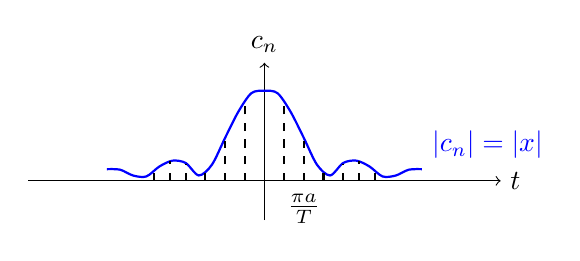
\begin{tikzpicture}
            % Define axis
            \draw[->] (-3,0) -- (3,0) node[right] {$t$};
            \draw[->] (0,-0.5) -- (0,1.5) node[above] {$\modulus{c_n}$};
            
            % Plot the function
            \draw[domain=-2:2, smooth, variable=\x, blue, thick] 
                plot ({\x}, {abs(0.3*sin(4*\x r)/\x)}) 
                node[above right] {$|c_n| = |\sinc{x}|$};

             % Labels for x-axis values
            \node[below] at (0.5, -0.05) {$\frac{\pi a}{T}$};
    
            % Vertical lines of the straight line
            \draw[thick,dashed] (-0.25, 0) -- (-0.25, 1);
            \draw[thick,dashed] (-0.5, 0) -- (-0.5, 0.5);
            \draw[thick,dashed] (-0.75, 0) -- (-0.75, 0.2);
            \draw[thick,dashed] (-1, 0) -- (-1, 0.22);
            \draw[thick,dashed] (-1.2, 0) -- (-1.2, 0.25);
            \draw[thick,dashed] (-1.4, 0) -- (-1.4, 0.1);
            \draw[thick,dashed] (0.25, 0) -- (0.25, 1);
            \draw[thick,dashed] (0.5, 0) -- (0.5, 0.5);
            \draw[thick,dashed] (0.75, 0) -- (0.75, 0.2);
            \draw[thick,dashed] (1, 0) -- (1, 0.22);
            \draw[thick,dashed] (1.2, 0) -- (1.2, 0.25);
            \draw[thick,dashed] (1.4, 0) -- (1.4, 0.1);
            
        \end{tikzpicture}
        \caption{Amplitude Spectrum, $\modulus{c_n}$}
        \label{fig:1.1.a}
    \end{subfigure}
    \hfill
    \begin{subfigure}[t]{0.45\textwidth}
        \centering
        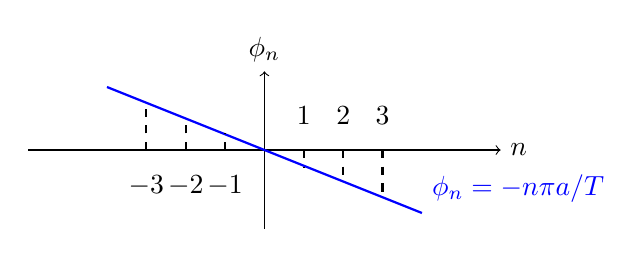
\begin{tikzpicture}
            % Define axis
            \draw[->] (-3,0) -- (3,0) node[right] {$n$};
            \draw[->] (0,-1) -- (0,1) node[above] {$\phi_n$};
            
            % Plot the function
            \draw[domain=-2:2, smooth, variable=\x, blue, thick] 
                plot ({\x}, {-0.4*\x)}) 
                node[above right] {$\phi_n = -n\pi a/T$};
    
            % Labels for x-axis values
            \node[below] at (-0.5, -0.2) {$-1$};
            \node[below] at (-1, -0.2) {$-2$};
            \node[below] at (-1.5, -0.2) {$-3$};
            \node[above] at (0.5, 0.2) {$1$};
            \node[above] at (1, 0.2) {$2$};
            \node[above] at (1.5, 0.2) {$3$};
    
            % Vertical lines of the straight line
            \draw[thick,dashed] (-0.5, 0) -- (-0.5, 0.22);
            \draw[thick,dashed] (-1, 0) -- (-1, 0.42);
            \draw[thick,dashed] (-1.5, 0) -- (-1.5, 0.62);
            \draw[thick,dashed] (0.5, 0) -- (0.5, -0.22);
            \draw[thick,dashed] (1, 0) -- (1, -0.42);
            \draw[thick,dashed] (1.5, 0) -- (1.5, -0.62);
            
        \end{tikzpicture}
    \caption{Phase Spectrum, $\phi_n$}
    \label{fig:1.1.b}
    \end{subfigure}
    \caption{Amplitude and Phase Spectrum [different shapes for each function $\f{x}$]}
    \label{fig:1.1}
\end{figure}
\subsubsection{The Two Domains}
\begin{itemize}
    \item \textbf{Waveform} is described in terms of behaviour in \textit{time}, $t$.
    \item \textbf{Spectrum} is described in terms of behaviour \textit{relative to frequency}, $\omega=2\pi f$.
    \item Since $t$ and $\omega$ form two domains of definition of our function, any information from one domain can be equally obtained within the other.
    \item For example, \textbf{power content} of periodic function $\f{t}$ of period $T$ defined in the \textit{time domain} and \textit{frequency domain} respectively:
    \begin{equation}
        \frac{1}{T}\intt{-T/2}{T/2}\bracket{\f{t}}^2dt\quad\text{and}\quad\summation{n=-\infty}{\infty}\modulus{c_n}^2
    \end{equation}
\end{itemize}
\subsubsection{Continuous Spectra}
\begin{itemize}
    \item In Fourier series, distance between neighbouring harmonics in complex spectra is the fundamental frequency $\omega_0=\frac{2\pi}{T}$.
    \item As $T\rightarrow\infty$, so $\omega_0\rightarrow 0$. Means as the period increase, the space between lines in the spectrum decrease and eventually merge into a continuous spectrum. So, for large $T$:
    \begin{align}
        n\omega_0\approx n\delta\omega,\quad\text{and as }T\rightarrow\infty\Rightarrow n\delta\omega\rightarrow\omega\\
        \text{where $\omega$}=\text{continuous frequency variable}\nonumber
    \end{align}
\end{itemize}
\begin{figure}[h]
    \centering
    \begin{subfigure}[t]{0.45\textwidth}
        \centering
        \begin{tikzpicture}
            % Define axis
            \draw[->] (-3,0) -- (3,0) node[right] {$t$};
            \draw[->] (0,-0.5) -- (0,1.5) node[above] {$\f{t}$};
            
             % Labels for x-axis values
            \node[below] at (-1, -0.025) {$-\frac{T}{2}$};
            \node[below] at (1, -0.05) {$\frac{T}{2}$};

            % Labels for y-axis values
            \node[above] at (0.2, 0.95) {$A$};
            
            % Plot straight line
            \draw[domain=-1:1, smooth, variable=\x, blue] 
            plot ({\x}, {1});
            \draw[domain=-3:-2, smooth, variable=\x, blue, dashed] 
            plot ({\x}, {1});
            \draw[domain=2:3, smooth, variable=\x, blue, dashed] 
            plot ({\x}, {1});
    
            % Vertical lines of the straight line
            \draw[thick,dashed] (-1, 0) -- (-1, 1);
            \draw[thick,dashed] (1, 0) -- (1, 1);
    
            % Vertical lines of other straight line
            \draw[thick,dashed] (-2, 0) -- (-2, 1);
            \draw[thick,dashed] (2, 0) -- (2, 1);
            
        \end{tikzpicture}
        \caption{Discrete time function, $\f{t}$}
        \label{fig:1.2.a}
    \end{subfigure}
    \hfill
    \begin{subfigure}[t]{0.45\textwidth}
        \centering
        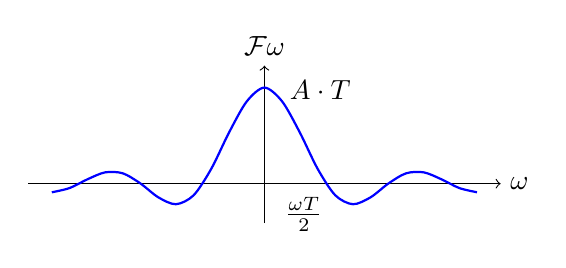
\begin{tikzpicture}
            % Define axis
            \draw[->] (-3,0) -- (3,0) node[right] {$\omega$};
            \draw[->] (0,-0.5) -- (0,1.5) node[above] {$\mathcal{F}\bracket{\omega}$};
            
            % Plot the function
            \draw[domain=-2.7:2.7, smooth, variable=\x, blue, thick] 
                plot ({\x}, {0.3*sin(4*\x r)/\x});

             % Labels for x-axis values
            \node[below] at (0.5, -0.05) {$\frac{\omega T}{2}$};

            % Labels for y-axis values
            \node[above right] at (0.2, 0.95) {$A\cdot T$};
            
        \end{tikzpicture}
    \caption{Continuous amplitude spectrum, $\F{\omega}$}
    \label{fig:1.2.b}
    \end{subfigure}
    \caption{Discrete and continuous spectrum [different shapes for each function $\f{t}$]}
    \label{fig:1.2}
\end{figure}
Using this result, we can derive the Fourier Transform equation.
\newpage
\subsection{Fourier Transform}
\subsubsection{Fourier's Integral Theorem}
\nicebox{0.9}{
        Given function $f\bracket{t}$ with derivatives $f'\bracket{t}$ where
        \begin{enumerate}
            \item $\f{t}$ and $f'\bracket{t}$ are piecewise continuous in every finite interval.
            \item $\f{t}$ is absolutely integrable in $ \bracket{\infty,-\infty}$, that is $\displaystyle\intt{-\infty}{\infty}\modulus{\f{t}}dt<\infty$ (finite).
        \end{enumerate}
}\vspace{0.5ex}
Fourier Transform, $\mathcal{F}\bracket{\omega}$:
\begin{equation}
    \mathcal{F}\bracket{\omega}=\frac{1}{\sqrt{2\pi}}\intt{-\infty}{\infty}\f{t}e^{-iwt}dt
\end{equation}
Inverse Fourier Transform, $f\bracket{\omega}$:
\begin{equation}
    f\bracket{t}=\frac{1}{\sqrt{2\pi}}\intt{-\infty}{\infty}\mathcal{F}\bracket{\omega}e^{i\omega t}d\omega
\end{equation}
\subsubsection{Properties of Fourier Transform}
\subsubsection*{1. Linearity}
\begin{align}
    \mathscr{F}\sbracket{\alpha_1f_1\bracket{t}+\alpha_2f_2\bracket{t}}&=\alpha_1\mathscr{F}\sbracket{f_1\bracket{t}}+\alpha_2\mathscr{F}\sbracket{f_2\bracket{t}}\\
    \text{where }\alpha_1,\alpha_2&=\text{any constants}\nonumber
\end{align}
\subsubsection*{2. Time Shifting}
If $\mathscr{F}\sbracket{\f{t}}=\mathcal{F}\bracket{\omega}$, then:
\begin{equation}
    \mathscr{F}\sbracket{\f{t-t_0}}=e^{i\omega t_0}\mathcal{F}\bracket{w}
\end{equation}
\subsubsection*{3. Frequency Shifting}
If $\mathscr{F}\sbracket{\f{t}}=\mathcal{F}\bracket{\omega}$, then:
\begin{equation}
    \mathscr{F}\sbracket{\f{t}e^{i\omega_0t}}=\mathcal{F}\bracket{\omega-\omega_0}
\end{equation}
\subsubsection*{4. Time Scaling}
If $\mathscr{F}\sbracket{\f{t}}=\mathcal{F}\bracket{\omega}$, then:
\begin{equation}
    \mathscr{F}\sbracket{\f{kt}}=\frac{1}{\modulus{k}}\mathcal{F}\bracket{\frac{\omega}{k}}
\end{equation}
\subsubsection*{5. Symmetry}
If $\mathscr{F}\sbracket{\f{t}}=\mathcal{F}\bracket{\omega}$, then:
\begin{equation}
    \mathscr{F}\sbracket{\mathcal{F}\bracket{t}}=\f{-\omega}
\end{equation}
\subsubsection*{6. Differentiation}
If $\f{t}\to0$ as $t\to\pm\infty$ and if $\mathscr{F}\sbracket{\f{t}}=\mathcal{F}\bracket{\omega}$, then:
\begin{equation*}
    \mathscr{F}\sbracket{f'\bracket{t}}=i\omega\mathcal{F}\bracket{\omega}
\end{equation*}
More generally:
\begin{equation}
    \mathscr{F}\sbracket{f^{\bracket{n}}\bracket{t}}=\bracket{i\omega}^n\mathcal{F}\bracket{\omega}
\end{equation}
\subsubsection{Alternative Forms of Fourier Transform}
Alternate form 1:
\begin{align}
    \f{t}&=\intt{-\infty}{\infty}\mathcal{F}\bracket{\omega}e^{i\omega t}d\omega\nonumber\\
    \mathcal{F}\bracket{\omega}&=\frac{1}{2\pi}\intt{-\infty}{\infty}\f{t}e^{-i\omega t}dt
\end{align}
Alternate form 2:
\begin{align}
        \f{t}&=\frac{1}{2\pi}\intt{-\infty}{\infty}\mathcal{F}\bracket{\omega}e^{i\omega t}d\omega\nonumber\\
        \mathcal{F}\bracket{\omega}&=\intt{-\infty}{\infty}\f{t}e^{-i\omega t}dt
\end{align}
Alternate form 3:
\begin{align}
        \f{t}&=\intt{-\infty}{\infty}\mathcal{F}\bracket{\omega}e^{i2\pi\omega t}d\omega\nonumber\\ \mathcal{F}\bracket{\omega}&=\intt{-\infty}{\infty}\f{t}e^{-i2\pi\omega t}dt
\end{align}
\subsection{Special Transforms}
\subsubsection{Odd, Even, Sine and Cosine}
If $\f{t}$ is odd or even, can use $\mathcal{F}_s$ and $\mathcal{F}_c$ respectively. Notice that values of \textit{odd} \& $\mathcal{F}_s$ and \textit{even} \& $\mathcal{F}_c$ are $\mathbb{C}$ and $\mathbb{R}$ respectively.\vspace{2ex}\\
Odd functions:
\begin{equation}
    \mathcal{F}\bracket{\omega}=-i\sqrt{\frac{2}{\pi}}\intt{0}{\infty}\f{t}\sinn{\omega t}dt
\end{equation}
Even functions:
\begin{equation}
    \mathcal{F}\bracket{\omega}=\sqrt{\frac{2}{\pi}}\intt{0}{\infty}\f{t}\coss{\omega t}dt
\end{equation}
Fourier Sine Transform $\mathcal{F}_s$:
\begin{equation}
    \mathcal{F}_s\bracket{\omega}=\sqrt{\frac{2}{\pi}}\intt{0}{\infty}\f{t}\sinn{\omega t}dt
\end{equation}
Fourier Cosine Transform $\mathcal{F}_c$:
\begin{equation}
    \mathcal{F}_c\bracket{\omega}=\sqrt{\frac{2}{\pi}}\intt{0}{\infty}\f{t}\coss{\omega t}dt
\end{equation}
Fourier Transform when $\f{t}=\e{-qt}$:
\begin{equation*}
    \mathcal{F}_s=\sqrt{\frac{2}{\pi}}\cdot\frac{\omega}{\omega^2+q^2}\quad\text{and}\quad\mathcal{F}_c=\sqrt{\frac{2}{\pi}}\cdot\frac{q}{\omega^2+q^2}
\end{equation*}
\subsubsection{Top-Hat Function}
Denoted by $\Pi_a\bracket{t}$ and is defined by:
\begin{equation}
    f\bracket{x}=
    \begin{cases}
        0, & \ \ \ \ \ \ \ \ t < -\frac{a}{2} \\
        \frac{1}{a}, & -\frac{a}{2} < t < \frac{a}{2}\\
        0, & \ \  \frac{a}{2} < t
    \end{cases}
\end{equation}
\noindent Fourier Transform $\F{\omega}$:
\begin{equation}
    \mathcal{F}\bracket{\omega}=\frac{1}{\sqrt{2\pi}}\sinc{\frac{\omega a}{2}}
\end{equation}
\begin{figure}[H]
    \centering
    \begin{subfigure}[t]{0.45\textwidth}
        \centering
        \begin{tikzpicture}
            % Define the axes
            \draw[->] (-3, 0) -- (3, 0) node[right] {$t$}; % x-axis
            \draw[->] (0, -0.5) -- (0, 1.5) node[above] {$f(t)$}; % y-axis
            
            % Labels for x-axis values
            \node[below] at (-1, 0) {$-\frac{a}{2}$};
            \node[below] at (1, 0) {$\frac{a}{2}$};
            
            % Horizontal line of the top-hat function
            \draw[thick,blue] (-1, 1) -- (1, 1);
            
            % Vertical lines of the top-hat function
            \draw[thick,dashed] (-1, 0) -- (-1, 1);
            \draw[thick,dashed] (1, 0) -- (1, 1);
            
            % Label the height of the top-hat function
            \node[left] at (1.5, 1) {$\frac{1}{a}$};
    
        \end{tikzpicture}
        \caption{Top-hat function, $\Pi_a\bracket{t}$}
        \label{fig:1.3.a}
    \end{subfigure}
    \hfill
    \begin{subfigure}[t]{0.45\textwidth}
        \centering
        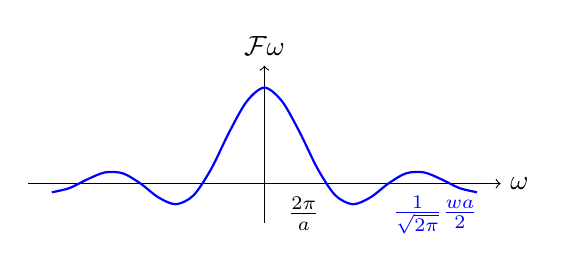
\begin{tikzpicture}
            % Define axis
            \draw[->] (-3,0) -- (3,0) node[right] {$\omega$};
            \draw[->] (0,-0.5) -- (0,1.5) node[above] {$\mathcal{F}\bracket{\omega}$};
            
            % Plot the function
            \draw[domain=-2.7:2.7, smooth, variable=\x, blue, thick] 
                plot ({\x}, {0.3*sin(4*\x r)/\x})
                node[below right] at (1.5,-.02) {$\frac{1}{\sqrt{2\pi}}\sinc{\frac{wa}{2}}$};

             % Labels for x-axis values
            \node[below] at (0.5, -0.05) {$\frac{2\pi}{a}$};
        \end{tikzpicture}
    \caption{Fourier transform of $\Pi_a\bracket{t}=\sinc{\frac{wa}{2}}$}
    \label{fig:1.3.b}
    \end{subfigure}
    \caption{Top-hat function, $\Pi_a$ and its fourier transform, $F\bracket{\omega}$}
    \label{fig:1.3}
\end{figure}
\noindent It is useful because it can be used to select any segment of any function. For example, to select segment $\bracket{\frac{\pi}{2},\frac{3\pi}{2}}$ of function $\coss{t}$:
\begin{align*}
    \Pi_\pi\bracket{t-\pi}&=
    \begin{cases}
        0, & \ \ \ \ \ \ \ \ t -\pi < -\frac{\pi}{2} \\
        \frac{1}{\pi}, & -\frac{\pi}{2} < t-\pi < \frac{\pi}{2}\\
        0, & \ \  \frac{\pi}{2} < t -\pi
    \end{cases}\\
    \Pi_\pi\bracket{t-\pi}&=
    \begin{cases}
        0, & \ \ \ \ \ \ \ t < \frac{\pi}{2} \\
        \frac{1}{\pi}, & \ \frac{\pi}{2} < t < \frac{3\pi}{2}\\
        0, &  \frac{3\pi}{2} < t 
    \end{cases}\\
    \pi\Pi_\pi\bracket{t-\pi}\coss{t}&=
    \begin{cases}
        \coss{t}, & \frac{\pi}{2} < t < \frac{3\pi}{2} \\
        0, & \text{otherwise} 
    \end{cases}
\end{align*}
\begin{figure}[H]
    \centering
        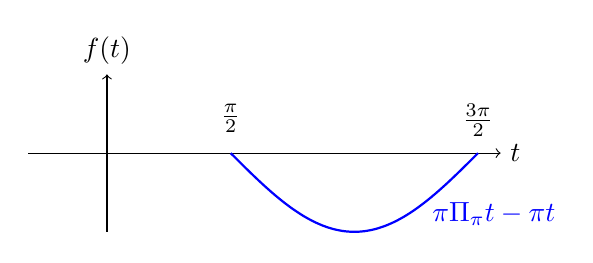
\begin{tikzpicture}
        % Define the axes
        \draw[->] (-1, 0) -- (5, 0) node[right] {$t$}; % x-axis
        \draw[->] (0, -1) -- (0, 1) node[above] {$f(t)$}; % y-axis
        
        % Labels for x-axis values
        \node[below] at (3.142/2, 0.75) {$\frac{\pi}{2}$};
        \node[below] at (3*3.142/2, 0.75) {$\frac{3\pi}{2}$};
        
        % Plot cos
        \draw[domain=3.142/2:3*3.142/2, smooth, variable=\x, blue, thick] 
            plot ({\x}, {cos(\x r))}) 
            node[below right] at (4,-0.5) {$\pi\Pi_\pi\bracket{t-\pi}\coss{t}$};
    \end{tikzpicture}
    \caption{Top-hat function used to select segment of $\coss{t}$.}
    \label{fig:1.4}
\end{figure}
\subsubsection{Dirac Delta Function}
Is a \textit{\textbf{unit area pulse}}. Often used to represent force acting for a very brief period of time.
\begin{equation}
    \lim\limits_{a \to 0}\intt{-\infty}{\infty}\{\Pi_a\bracket{t}\}dt=\intt{-\infty}{\infty}\delta\bracket{t}dt=1
\end{equation}
Therefore, we accept validity of integral:
\begin{equation}
    \intt{-\infty}{\infty}\f{t}\delta\bracket{t-t_0}dt=\f{t_0}
\end{equation}
Fourier Transform $\F{\omega}$:
\begin{equation}
    \mathcal{F}\bracket{\omega}=\frac{1}{\sqrt{2\pi}}
\end{equation}
Like the top-hat function, selects only \textit{part of $\f{t}$} over which is non-zero, namely at $t=t_0$.
\begin{figure}[h]
    \centering
    \begin{subfigure}[t]{0.45\textwidth}
        \centering
        \begin{tikzpicture}
            % Axes
            \draw[->] (-0.5,0) -- (4,0) node[below right] {$t$}; % x-axis
            \draw[->] (0,-0.5) -- (0,2) node[above] {$\delta(t)$}; % y-axis
        
            % Dirac delta impulse
            \draw[thick, ->, blue] (0, 0) -- (0, 1.5); % Arrow for the delta function
            \draw[thick, ->, red] (2, 0) -- (2, 1.5); % Arrow for shifted delta function
            \node[above] at (2, 1.5) {$\delta(t - t_0)$}; % Label the impulse
        
            % Label for t0 and y-axis
            \node[below] at (2, 0) {$t_0$};
            \node[above left] at (0, 1.4) {$\infty$};
            
        \end{tikzpicture}
        \caption{Dirac delta function, $\delta\bracket{t}$}
        \label{fig:1.5.a}
    \end{subfigure}
    \hfill
    \begin{subfigure}[t]{0.45\textwidth}
        \centering
        \begin{tikzpicture}
            % Define axis
            \draw[->] (-3,0) -- (3,0) node[right] {$\omega$};
            \draw[->] (0,-0.5) -- (0,2) node[above] {$\mathcal{F}\bracket{\omega}$};
            
            % Plot the function
            \draw[domain=-2.7:2.7, smooth, variable=\x, blue, thick] 
                plot ({\x}, {0.6})
                node[above] at (2,0.6) {$\frac{1}{\sqrt{2\pi}}$};

             % Labels for x and y axis values
            \node[above left] at (0, 0.6) {$\frac{1}{\sqrt{2\pi}}$};
            
        \end{tikzpicture}
    \caption{Fourier transform of $\delta\bracket{t}=\frac{1}{\sqrt{2\pi}}$}
    \label{fig:1.5.b}
    \end{subfigure}
    \caption{Dirac delta function, $\delta\bracket{t}$ and its fourier transform, $F\bracket{\omega}$}
    \label{fig:1.5}
\end{figure}
\subsubsection{Triangle Function}
Defined by the equation:
\begin{equation}
    \Lambda_a\bracket{t}=
    \begin{cases}
        \bracket{a+t}/a^2, & -a < t < 0 \\
        \bracket{a-t}/a^2, & \ \ 0 < t < a\\
        0, & \ \ \ \ \ \ \ \modulus{t} > a
    \end{cases}\\
\end{equation}
Fourier Transform $\F{\omega}$:
\begin{equation}
    \mathcal{F}\bracket{\omega}=\frac{1}{\sqrt{2\pi}}\text{sinc}^2\bracket{\frac{\omega}{2}}
\end{equation}
\begin{figure}[h]
    \centering
    \begin{subfigure}[t]{0.45\textwidth}
        \centering
        \begin{tikzpicture}
            % Define the axes
            \draw[->] (-3, 0) -- (3, 0) node[right] {$t$}; % x-axis
            \draw[->] (0, -0.5) -- (0, 1.5) node[above] {$\Lambda_0(t)$}; % y-axis
            
            % Labels for x-axis values
            \node[below] at (-1, -0.2) {$-a$};
            \node[below] at (1, -0.2) {$a$};
            \node[right] at (0.2, 1) {$\frac{1}{a}$};
            
            % Plot cos
            \draw[domain=-1:0, smooth, variable=\x, blue, thick] 
                plot ({\x}, {\x + 1});
            \draw[domain=0:1, smooth, variable=\x, blue, thick] 
                plot ({\x}, {-\x + 1});
        \end{tikzpicture}
        \caption{Triangle function $\Lambda_a\bracket{t}$.}
        \label{fig:1.6.a}
    \end{subfigure}
    \hfill
    \begin{subfigure}[t]{0.45\textwidth}
        \centering
        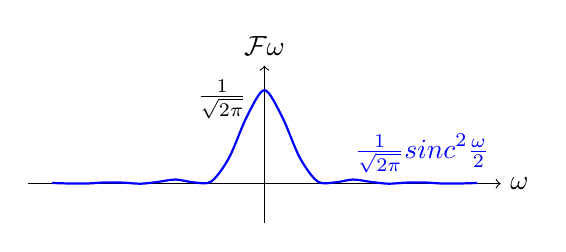
\begin{tikzpicture}
            % Define axis
            \draw[->] (-3,0) -- (3,0) node[right] {$\omega$};
            \draw[->] (0,-0.5) -- (0,1.5) node[above] {$\mathcal{F}\bracket{\omega}$};
            
            % Plot the function
            \draw[domain=-2.7:2.7, smooth, variable=\x, blue, thick] 
                plot ({\x}, {(0.07*(sin(4*\x r)/\x)^2})
                node[above] at (2,0) {$\frac{1}{\sqrt{2\pi}}\text{sinc}^2\bracket{\frac{\omega}{2}}$};

             % Labels for x and y axis values
            \node[above left] at (-0.1, 0.7) {$\frac{1}{\sqrt{2\pi}}$};
            
        \end{tikzpicture}
    \caption{Fourier transform of $\Lambda_a\bracket{t}=\text{sinc}^2\bracket{\frac{w}{2}}$}
    \label{fig:1.6.b}
    \end{subfigure}
    \caption{Triangle function, $\Lambda_a\bracket{t}$ and its fourier transform, $F\bracket{\omega}$}
    \label{fig:1.6}
\end{figure}
\subsubsection{Heaviside Unit Step Function}
Is defined as $u\bracket{t}$ where:
\begin{equation}
    u\bracket{t}=
    \begin{cases}
        0, & t < 0\\
        1, & t > 0 
    \end{cases}
\end{equation}
Fourier Transform $\mathcal{F}\bracket{\omega}$:
\begin{align}
    \mathcal{F}\bracket{\omega}&=\frac{1}{\sqrt{2\pi}i\omega}-\cbracket{1-\lim\limits_{t\to\infty}\sbracket{e^{-i\omega t}}}\nonumber\\
    &=\frac{1}{\sqrt{2\pi}}\cbracket{\pi\delta\bracket{\omega}+\frac{1}{j\omega}}
\end{align}
\begin{figure}[H]
    \centering
        \begin{tikzpicture}
        % Define the axes
        \draw[->] (-3, 0) -- (3, 0) node[right] {$t$}; % x-axis
        \draw[->] (0, -1) -- (0, 1) node[above] {$f(t)$}; % y-axis
        
        % Plot cos
        \draw[domain=-2:0, smooth, variable=\x, blue, thick] 
            plot ({\x}, {-0.5})
            node[above left] {-1};
        \draw[domain=0:2, smooth, variable=\x, blue, thick] 
            plot ({\x}, {0.5})
            node[above right] at (0,0) {1};
            
    \end{tikzpicture}
    \caption{Heaviside unit step function $u\bracket{t}$}
    \label{fig:1.7}
\end{figure}\vspace{-5ex}
\subsection{Convolution}
Convolution of two functions $\f{t}$ and $g\bracket{t}$ defined as:
\begin{equation}
    \boxed{\f{t}*g\bracket{t}=\intt{-\infty}{\infty}\f{x}g\bracket{t-x}dx=h\bracket{t}}
\end{equation}
\begin{center}
    where $*$ denotes convolution
\end{center}\vspace{-2.5ex}
\subsubsection{Properties of Convolution}
\nicebox{0.6}{
\begin{enumerate}
    \item Commutativity: $f*g=g*f$
    \item Associativity: $f*\bracket{g*h}=\bracket{f*g}*h$
    \item Distributivity: $f*\bracket{g+h}=\bracket{f*g}+\bracket{f*h}$
\end{enumerate}
}
\subsubsection{Convolution Theorem}
If $\F{\omega}$ and $\mathcal{G}\bracket{\omega}$ are Fourier transforms of $\f{t}$ and $g\bracket{t}$ respectively, then:
\begin{enumerate}
    \item Fourier transform of the \textbf{convolution of} $\mathbf{\f{t}}$ and $\mathbf{g\bracket{t}}$ is \textit{equal} to the \textit{product of the individual Fourier transforms}:
    \begin{align}
        \mathscr{F}\sbracket{\f{t}*g\bracket{t}}&=\sqrt{2\pi}\F{\omega}\mathcal{G}\bracket{\omega}\\
        \mathscr{F}^{-1}\sbracket{\F{\omega}\mathcal{G}\bracket{\omega}}&=\frac{1}{\sqrt{2\pi}}\sbracket{\f{t}*g\bracket{t}}
    \end{align}
    \item Fourier transform of the \textbf{product of} $\mathbf{\f{t}g\bracket{t}}$ is \textit{equal} to the \textit{convolution of the individual Fourier transforms}:
    \begin{align}
        \mathscr{F}\sbracket{\f{t}g\bracket{t}}&=\frac{1}{\sqrt{2\pi}}\F{\omega}*\mathcal{G}\bracket{\omega}\\
        \mathscr{F}^{-1}\sbracket{\F{\omega}*\mathcal{G}\bracket{\omega}}&=\sqrt{2\pi}\f{t}g\bracket{t}
    \end{align}
\end{enumerate}
They provide useful methods to find inverse transforms, especially in \textit{Laplace Transforms.}
\begin{table}[h]
    \centering
    \renewcommand{\arraystretch}{2.6}
    \caption{Table of Transformations}
    \label{table:1.1}
    \begin{tabular}{|c|m{7cm}|m{7cm}|}\hline
       Num.& \centering Fourier, $\f{t}$ & \centering Fourier Transform, $\F{\omega}$ \arraybackslash \\ \hline\hline
       1.&$\f{t}=\begin{cases}
           1 & \text{if }-a/2<t<a/2\\
           0 & \text{otherwise}
       \end{cases}$ & $\F{\omega}=\displaystyle\frac{a}{\sqrt{2\pi}}\sinc{\omega a/2}$\\ \hline
       2.&$\f{t}=\begin{cases}
           1 & \text{if }0<t<a\\
           0 & \text{otherwise}
       \end{cases}$ & $\F{\omega}=\displaystyle\frac{ae^{-i\omega a/2}}{\sqrt{2\pi}}\sinc{\omega a/2}$\\ \hline
       3.&$\Pi_a\bracket{t}=\begin{cases}
           1/a & \text{if }-a/2<t<a/2\\
           0 & \text{otherwise}
       \end{cases}$  & $\F{\omega}=\displaystyle\frac{1}{\sqrt{2\pi}}\sinc{\omega a/2}$\\\hline
       4.&$\f{t}=u\bracket{t}$ & $\F{\omega}=\displaystyle\frac{1}{\sqrt{2\pi}}\cbracket{\pi\delta\bracket{\omega}+\frac{1}{iw}}$\\\hline
       5.&$\f{t}=e^{-at}\cdot u\bracket{t}$ & $\F{\omega}=\displaystyle\frac{1}{\sqrt{2\pi}}\cbracket{\pi\delta\bracket{\omega+a}+\frac{1}{iw}}$\\\hline
       6.&$\f{t}=te^{-at}\cdot u\bracket{t}$ & $\F{\omega}=\displaystyle\frac{1}{\sqrt{2\pi}\bracket{a+iw}^2}$\\\hline
       7.&$\f{t}=\delta\bracket{t}$ & $\F{\omega}=\displaystyle\frac{1}{\sqrt{2\pi}}$\\ \hline
    \end{tabular}
\end{table}
\newpage
\subsection{Miscellaneous}
\begin{table}[h]
    \centering
    \renewcommand{\arraystretch}{2.6}
    \caption{Table of Cosine and Sine Integrals}
    \label{table:1.2}
    \begin{tabular}{|c|m{10cm}|}\hline
       Num.& \centering Cosine and Sine Integrals (Period, $L$)\arraybackslash \\ \hline\hline
       1.&$\displaystyle\intt{-L}{L}\coss{\frac{n\pi x}{L}}dx=0$\\
       2.&$\displaystyle\intt{-L}{L}\sinn{\frac{n\pi x}{L}}dx=0$\\
       3.&$\displaystyle\intt{-L}{L}\cos^2\bracket{\frac{n\pi x}{L}}dx=L$\\
       4.&$\displaystyle\intt{-L}{L}\sin^2\bracket{\frac{n\pi x}{L}}dx=L$\\
       5.&$\displaystyle\intt{-L}{L}\coss{\frac{m\pi x}{L}}\coss{\frac{n\pi x}{L}}dx=\begin{cases}
           0 & \text{if }m\neq n\\
           L & \text{if }m=n
       \end{cases}$\\
       6.&$\displaystyle\intt{-L}{L}\sinn{\frac{m\pi x}{L}}\sinn{\frac{n\pi x}{L}}dx=\begin{cases}
           0 & \text{if }m\neq n\\
           L & \text{if }m=n
       \end{cases}$\\
       7.&$\displaystyle\intt{-L}{L}\cos{\frac{m\pi x}{L}}\sinn{\frac{n\pi x}{L}}dx=0$\\ \hline
    \end{tabular}
\end{table}
\newpage